\section{System's Perspective} 

\subsection{Design \& Architecture}
%Should contain a description and illustration of the design and architecture of our ITU-MiniTwit system.

%- What is our overarching architecture?
%- Have we made any design choices?
%- How is this best illustrated? Diagram?

%terraform og hvordan det bør sættes op?

We chose to rewrite the MiniTwit application to C\#. C\# has a nice web framework, Blazor, which allows us to write all our code using the same language. Our application depends on a few NuGet packages.

\begin{center}
\begin{tabular}{|c|p{0.6\linewidth}|}
    \hline
    Identity Server & An easy and secure way of managing users. \\
    \hline
    prometheus-net & Sets up the /metrics endpoints for Prometheus. \\
    \hline
    Serilog.Sinks.ElasticSearch & Gives Serilog a log sink for ElasticSearch, letting it send logs directly to ElastickSearch \\
    \hline
\end{tabular}
\end{center}

\begin{wrapfigure}{r}{0.4\textwidth}
    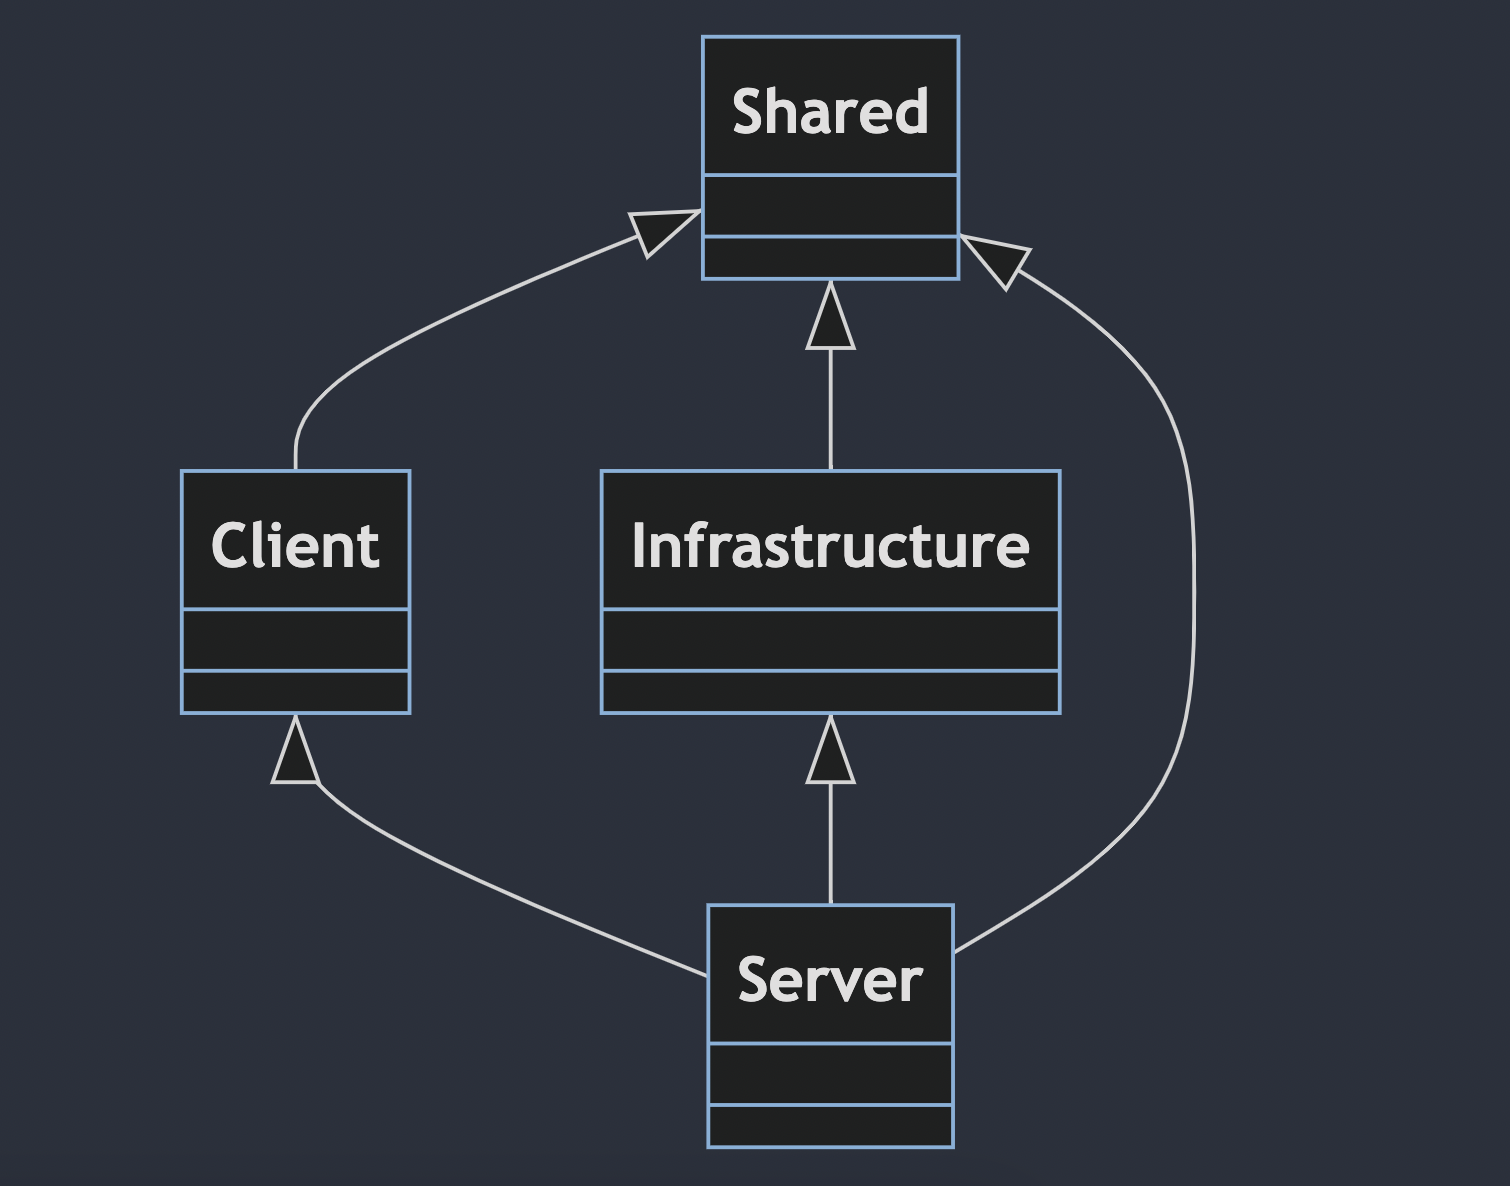
\includegraphics[width=0.9\linewidth]{Images/onionStructure.png} 
    \caption{Project dependency graph}
    \label{fig:projectDependencyGraph}
\end{wrapfigure}

We aimed to get a simple and maintainable system architecture, by utilizing as few different tools as possible and using software architectural patterns. The patterns we chose to strive for have been Clean architecture, Repository pattern, and client-server. We use several other patterns too, but we don't consider them something we strive for, as they are simply a byproduct of the tools and framework we use. We achieve Clean architecture by having our code split into 4 C\# projects. One project (Shared) for our data transfer objects (DTO's) and repository interfaces, so we will be able to mock our repositories without a dependency on them. A second project (Infrastructure) is for the repositories, database context, and models for the database schema, where the repositories depend on the S. The third project 

ef core






\subsection{Dependencies}
%Should contain a description and illustration of all dependencies of our ITU-MiniTwit system on all levels of abstraction and development stages. That is, list and briefly describe all technologies and tools you applied and depend on.


\begin{figure}[H]
    \centering
    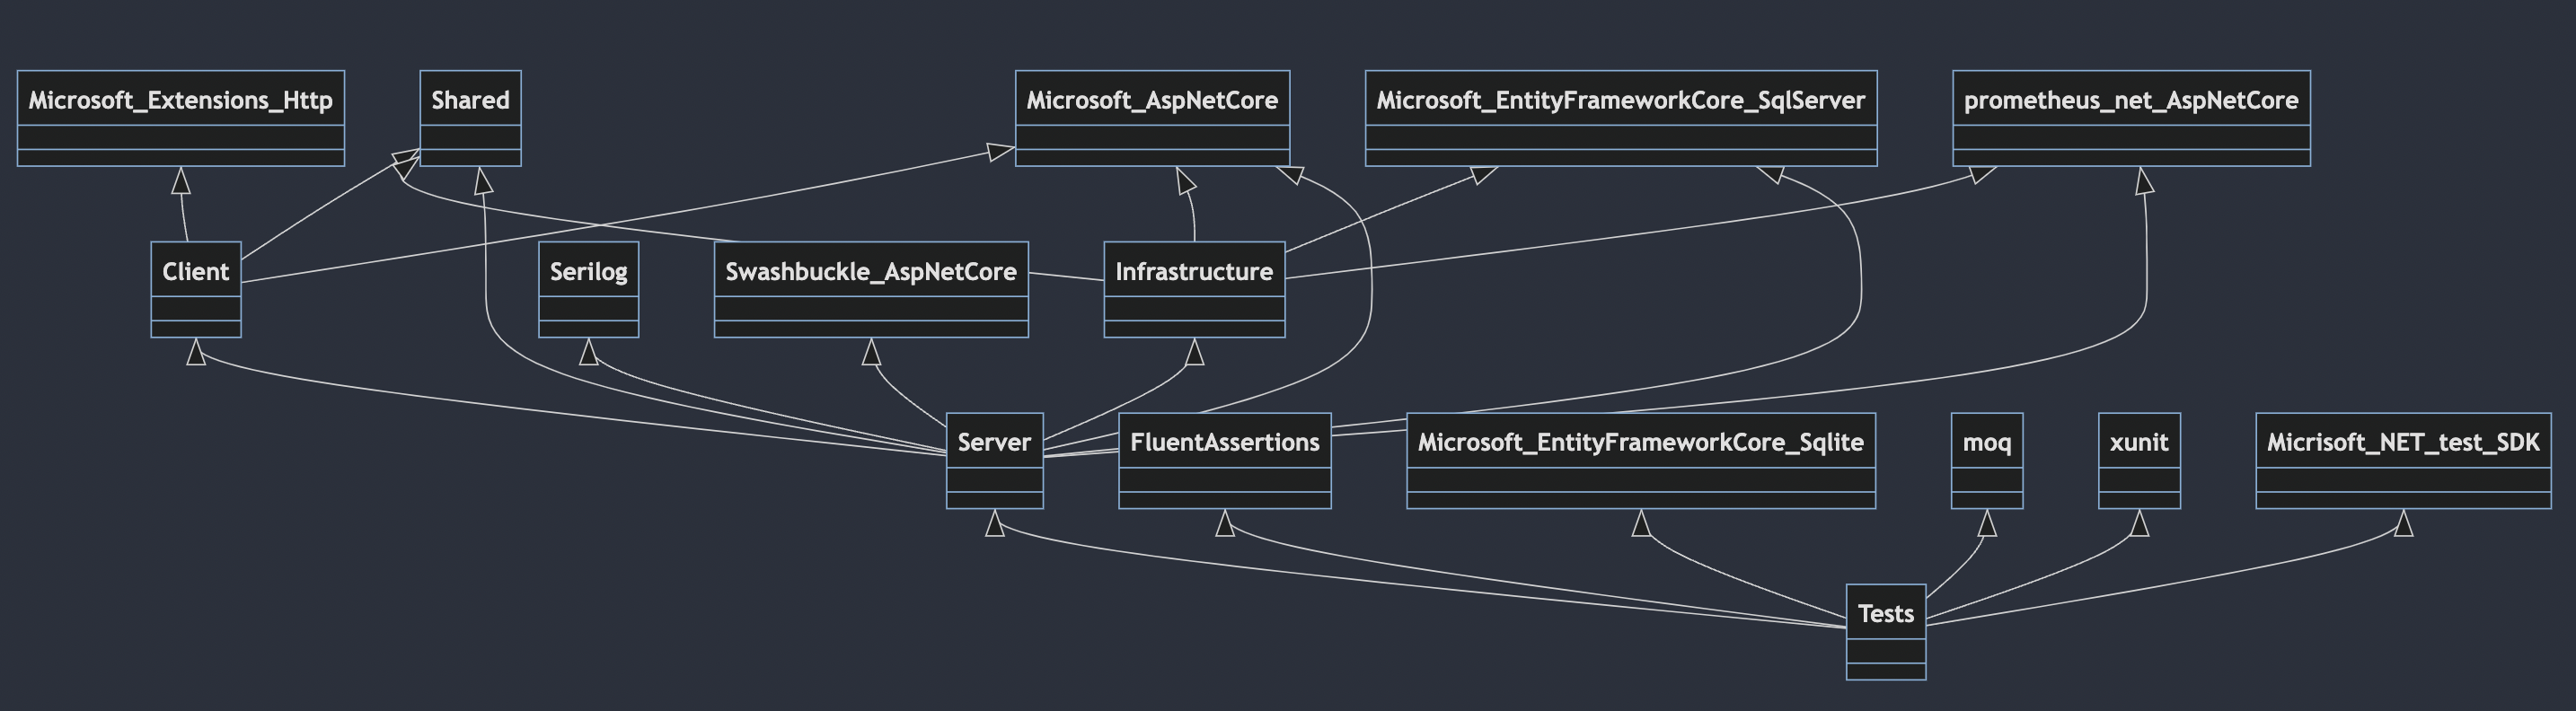
\includegraphics[width = 15.0cm, height = 5.0cm]{Images/dependencies2.png}
    \caption{Package dependency graph}
    \label{fig:packageDependencyGraph}
\end{figure}

Below are the dependencies for the deployement level. 

\begin{wrapfigure}{r}{0.4\textwidth}
    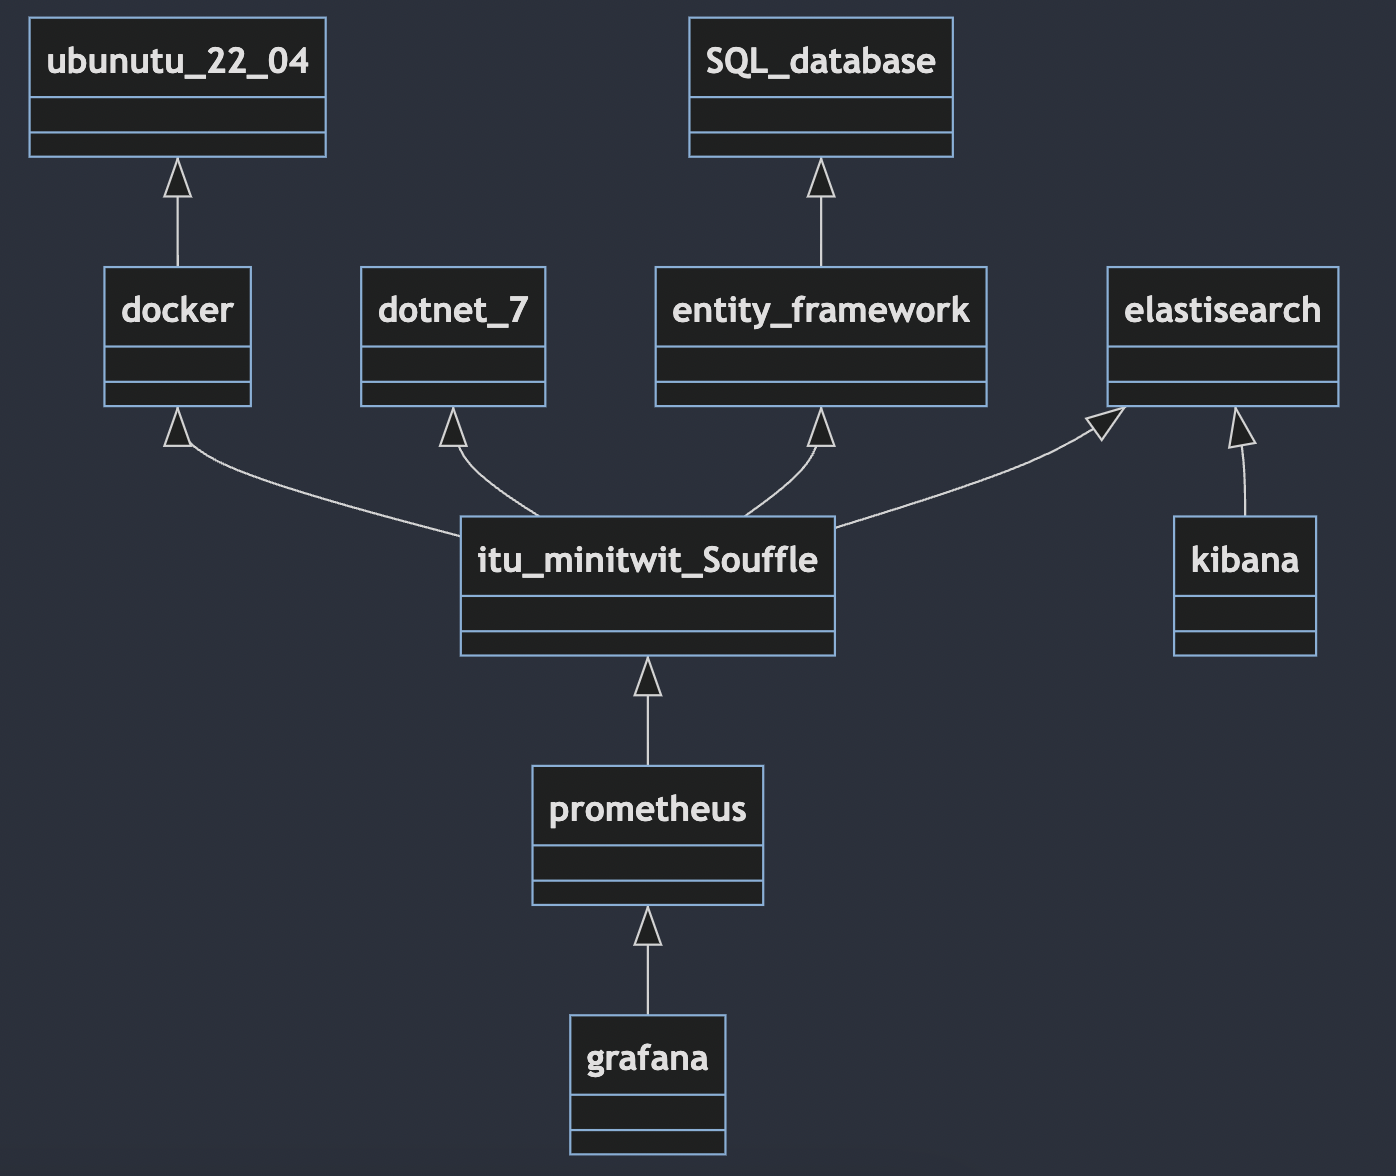
\includegraphics[width=0.9\linewidth]{Images/application_dependencies.png} 
    \caption{Application dependency graph}
    \label{fig:ApplicationDependencyGraph}
\end{wrapfigure}

text here describing dependencies
make use of elastisearch that displays 


%- What are the levels of abstraction?
%- What are the development stages? Early- Mid- Late?
%- Easiest way to graph all dependencies? Debtree, pipdebtree?

\subsection{Important Subsystem Interactions}
%Should contain a description and illustration of important interactions of subsystems.
%What interactions do we have?

Our applications main mode of subsystem interaction is through communication via APIs. It's through the endpoints that the API exposes, that the systemusers interacts with our program. Our client-side part of MiniTwit is written in Blazor WebAssembly. It compiles our different razor-pages into a single dll (or Single page app). Single page applications are faster at loading, partly because data can be fetched in the background and because full page reloads are rare. All this is made possible through the web API that we have defined. Our application uses this API to request data or perform server-side operations triggered by the user.  



%- Which of these do we consider important?

\subsection{Current System State}
%Describe the current state of our system, for example using results of static analysis and quality assessments.

In our system, we use static analysis tools such as Lint Code Base, Snyk and MegaLinter to identify and reduce possible code smells, such as duplicated code segments and long methods, which may affect maintainability and readability. 
For instance the Lint Code Base identified code duplication in our UserRepository.cs class which resulted in a refactoring of the code in order to improve code quality. Hence by making use of the static analysis tools and additionally code reviews we ensure that our codebase follows coding standards and best practices.
A penetration test has been performed in order to asses the systems security quality. The test showed that there overall weren't any severe warnings but some security issues were detected and sebsequently added as github issues is order to fix them. 


%%det her er link til rejected Pull request: https://github.com/PatrickMatthiesen/Souffle-MiniTwit/actions/runs/4542608958/jobs/8006236624


- How do you describe a system state?
- Do we have any static analysis or quality assessment?
- If no, how do we get it?
- What is the current state of our system?
- What is an example of an earlier system state?

\subsection{License}
Describe briefly, if the license that we have chosen for our project is actually compatible with the licenses of all our direct dependencies. 

-

Double check that for all the weekly tasks (those listed in the schedule) we include the corresponding information.

- What license do we have? MIT?
- How do we check compatibility?
- I don't understand "Double check" thing, what is the corresponding information?